\documentclass[a4,useAMS,usenatbib,usegraphicx,12pt]{article}
%External Packages and personalized macros
%=========================================================================
%		EXTERNAL PACKAGES
%=========================================================================
\usepackage[round]{natbib}
\usepackage[margin=3cm]{geometry}
\usepackage{hyperref}
\usepackage{times}
\usepackage{amsmath} 
\usepackage{amssymb}
\usepackage{graphicx}
\usepackage{array, xcolor, lipsum, bibentry}
\usepackage[nottoc, notlof, notlot]{tocbibind}

\definecolor{lightgray}{gray}{0.8}
\newcolumntype{L}{>{\raggedleft}p{0.14\textwidth}}
\newcolumntype{R}{p{0.8\textwidth}}
\newcommand\VRule{\color{lightgray}\vrule width 0.5pt}

\usepackage{booktabs}% http://ctan.org/pkg/booktabs
\newcommand{\tabitem}{~~\llap{\textbullet}~~}

%=========================================================================
%		INTERNAL MACROS
%=========================================================================
% To highlight comments 
\definecolor{red}{rgb}{1,0.0,0.0}
\newcommand{\red}{\color{red}}
\definecolor{darkgreen}{rgb}{0.0,0.5,0.0}
\newcommand{\SRK}[1]{\textcolor{darkgreen}{\bf SRK: \textit{#1}}}
\newcommand{\SRKED}[1]{\textcolor{darkgreen}{\bf #1}}

\newcommand{\LCDM}{$\Lambda$CDM~}
\newcommand{\beq}{\begin{eqnarray}}  
\newcommand{\eeq}{\end{eqnarray}}  
\newcommand{\zz}{$z\sim 3$} 
\newcommand{\apj}{ApJ}  
\newcommand{\apjs}{ApJS}  
\newcommand{\apjl}{ApJL}  
\newcommand{\aj}{AJ}  
\newcommand{\mnras}{MNRAS}  
\newcommand{\mnrassub}{MNRAS accepted}  
\newcommand{\aap}{A\&A}  
\newcommand{\aaps}{A\&AS}  
\newcommand{\araa}{ARA\&A}  
\newcommand{\nat}{Nature}  
\newcommand{\physrep}{PhR}
\newcommand{\pasp}{PASP}    
\newcommand{\pasj}{PASJ}    
\newcommand{\avg}[1]{\langle{#1}\rangle}  
\newcommand{\ly}{{\ifmmode{{\rm Ly}\alpha}\else{Ly$\alpha$}\fi}}
\newcommand{\hMpc}{{\ifmmode{h^{-1}{\rm Mpc}}\else{$h^{-1}$Mpc }\fi}}  
\newcommand{\hGpc}{{\ifmmode{h^{-1}{\rm Gpc}}\else{$h^{-1}$Gpc }\fi}}  
\newcommand{\hmpc}{{\ifmmode{h^{-1}{\rm Mpc}}\else{$h^{-1}$Mpc }\fi}}  
\newcommand{\hkpc}{{\ifmmode{h^{-1}{\rm kpc}}\else{$h^{-1}$kpc }\fi}}  
\newcommand{\hMsun}{{\ifmmode{h^{-1}{\rm {M_{\odot}}}}\else{$h^{-1}{\rm{M_{\odot}}}$}\fi}}  
\newcommand{\hmsun}{{\ifmmode{h^{-1}{\rm {M_{\odot}}}}\else{$h^{-1}{\rm{M_{\odot}}}$}\fi}}  
\newcommand{\Msun}{{\ifmmode{{\rm {M_{\odot}}}}\else{${\rm{M_{\odot}}}$}\fi}}  
\newcommand{\msun}{{\ifmmode{{\rm {M_{\odot}}}}\else{${\rm{M_{\odot}}}$}\fi}}  
\newcommand{\lya}{{Lyman$\alpha$~}}
\newcommand{\clara}{{\texttt{CLARA}}~}
\newcommand{\rand}{{\ifmmode{{\mathcal{R}}}\else{${\mathcal{R}}$ }\fi}}  


%MY COMMANDS #############################################################
\newcommand{\sub}[1]{\mbox{\scriptsize{#1}}}
\newcommand{\dtot}[2]{ \frac{ d #1 }{d #2} }
\newcommand{\dpar}[2]{ \frac{ \partial #1 }{\partial #2} }
\newcommand{\pr}[1]{ \left( #1 \right) }
\newcommand{\corc}[1]{ \left[ #1 \right] }
\newcommand{\lla}[1]{ \left\{ #1 \right\} }
\newcommand{\bds}[1]{\boldsymbol{ #1 }}
\newcommand{\oiint}{\displaystyle\bigcirc\!\!\!\!\!\!\!\!\int\!\!\!\!\!\int}
\newcommand{\mathsize}[2]{\mbox{\fontsize{#1}{#1}\selectfont $#2$}}
\newcommand{\eq}[2]{\begin{equation} \label{eq:#1} #2 \end{equation}}
\newcommand{\lth}{$\lambda_{th}$ }
%#########################################################################

\setlength\parindent{0pt}
 
\title{{\textbf{Research Proposal for a Master Thesis in Physics}}\\ 
				Verifying the VPH scheme in Galaxy Formation\\ 
				\color{black}\rule{15cm}{0.5mm}}
\author{Sebastian Bustamante Jaramillo}
\date{}
  
\begin{document}
\maketitle
\begin{center}
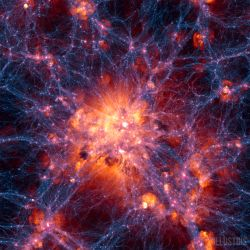
\includegraphics[trim = 0mm 3.5cm 0mm 3.0cm, clip, keepaspectratio=true,
width=0.7\textheight]{Presentation1.png}
\tiny{Time evolution of a gas cloud in a supersonic wind using a \VPH\ scheme.
Taken from \citep{Hess10}}
\end{center}
\tableofcontents
 
\newpage 

%============================================================================== 
\section{General Information}
\small
\subsection*{Information of the Student}
\begin{tabular}{L!{\VRule}R}
\bf Name		& Sebastian Bustamante Jaramillo\\
\bf Degree		& B.Sc. in Physics, Universidad de Antioquia (2013)\\
\bf E-mail 1	& macsebas33 \textit{at} gmail.com (personal)\\
\bf E-mail 2	& sebastian.bustamante \textit{at} udea.edu.co (academic)\\
\end{tabular}

\vspace{10pt}

More detailed information of the applicant can be found here \url{http://goo.gl/BPZGzK}

\vspace{15pt}  

\subsection*{Information of the Project}
\begin{tabular}{L!{\VRule}R}
\bf Title		& \bf Verifying the VPH scheme in Galaxy Formation\\
\bf Field		& Cosmology, Astrophysics, Physical Sciences \\
\bf Advisor 1	& Professor Juan Carlos Munoz-Cuartas. Universidad de Antioquia, Colombia.\\
\bf University	& Universidad de Antioquia, Master of Physics program \\
\bf Time Frame	& 2 years \\
\end{tabular}
\normalsize
%==============================================================================

%==============================================================================
\section{Abstract}
%==============================================================================
\newpage


%==============================================================================
\section{Introduction}
%==============================================================================
As we understand more deeply the physical processes involved in astrophysical 
phenomena, it becomes necessary to compute complex interactions of a ever 
increasing number of single components. Some prominent examples include 
the large-scale Universe, galaxy evolution, stellar interior, star formation 
and protoplanetary disk dynamics. A common aspect of these examples is that all 
of them can be regarded basically as a fluid mechanic problem.

\

Although the development of analytical approaches has demonstrated to be a
valuable resource for studying these processes, their increasing complexity 
makes necessary to invoke numerical solutions as a more feasible alternative. 
For this purpose, two different families of hydrodynamics solvers has been 
explored and widely used by the astrophysical community. First, a family of 
moving-mesh-based techniques (e.g. \textit{Smoothed Particle Hydrodynamics} 
\SPH\ \citep{Monaghan92}, \textit{Voronoi Particle Hydrodynamics} \VPH\ 
\citep{Hess10}), and a second family of fixed-mesh-based techniques (e.g.
\textit{Adaptive Mesh Refinement} \texttt{AMR} \citep{Berger89}).

\

Due to the Lagrangian character of moving-mesh methods, techniques like \SPH\ 
are easily implemented on a computer. Furthermore, as the physical system 
evolves, the mass particles naturally move into higher density regions, 
providing a self-adjusting spatial resolution. Nevertheless, \SPH\ has been 
shown to produce spurious suppression of fluid instabilities due to its 
kernel-based density estimator, making it unsuitable to model some of the 
dynamics accurately. On the other hand, fixed-mesh methods like \AMR\ are more 
efficient for capturing shock dynamics. However, due to the conservative nature 
of the hydrodynamical equations, a fixed mesh causes a lack of Galilean 
invariance. Furthermore, the sampling of physical properties over the grid 
introduces spurious vorticity to the fluid, making this technique poor suitable 
for studying turbulent flows.

\

A completely new approach to solve hydrodynamical problems was introduced by 
\citet{Springel10} and implemented into the \AREPO\ code. It combines the 
strengths of \AMR\ and \SPH\ but overcomes many of their weaknesses, hence it 
can be though as a mixed technique. \AREPO\ uses a moving mesh based on a 
Voronoi tessellation defined over a set of particles that represents the fluid. 
The geometry of the mesh resembles very closely that of the point distribution,
retaining the self-adaptivity inherent of \SPH\ and also keeping a grid to 
capture shocks like \AMR\ does. These features make \AREPO\ highly accurate for
simulating a wide range of hydrodynamical problems. Nevertheless, there is a 
price to pay for this accuracy, \AREPO\ demands a huge computing time as 
compared with \SPH\ and even \AMR.

\

A very interesting alternative was introduced by \citet{Hess10}, i.e. the 
\textit{Voronoi Particle Hydrodynamics} \VPH\ technique. This approach consists
of an implementation of \SPH\ with a modified density estimator based on the  
\textit{Voronoi Tessellation Field Estimator} \VTFE. The new estimator
has demonstrated to improve substantially the spurious suppression of fluid 
instabilities as well as retaining the computational efficiency of the original 
formulation.

\

Finally, galaxy evolution and large-scale structure formation are very rich 
astrophysical scenarios where a plethora of hydrodynamical processes can be 
found and studied. In this fashion, cosmological simulations are quite suitable 
for performing detailed physical and computational comparisons of all 
above-mentioned techniques. It is especially interesting to quantify the 
computational performance of the \VPH\ technique in terms of its physical 
accuracy as compared with the classic approaches and \AREPO.



%==============================================================================
\section{Objectives}
%==============================================================================
\subsection*{General Objective}
Quantifying the computational performance of the \VPH\ technique in terms of 
its physical accuracy for a cosmological setup.


\subsection*{Specific Objectives}
\begin{itemize}
\item Evaluating the physical accuracy provided by \VPH\ for a cosmological 
setup as compared with \AMR, \SPH\ and \AREPO.
\item Exploring and quantifying the differences between \VPH\ and \AMR\ for 
describing shock dynamics in specific hydrodynamical instabilities.
\item Exploring and quantifying the differences of \VPH\ and \SPH\ for 
describing turbulent flows.
\item Measuring the computational performance of \VPH\ as compared with \AREPO.
\end{itemize}


%==============================================================================
\section{Theoretical Framework}
%==============================================================================


%==============================================================================
\section{Methodology}
%==============================================================================
The proposed project is subject to a M.Sc. study and will cover the following 
steps:


\begin{itemize}
\item[\checkmark] \textit{First, a bibliographic review of the original papers 
of the discussed methods will be done. Also a review of previous comparison 
projects.}
\end{itemize}


Before carrying out our enterprise in quantifying the performance of \VPH\ over
cosmological setups, it is necessary to understand deeply the foundations of 
the classic approaches. At this point, a detailed bibliographic review of the 
original papers (for \SPH, \AMR, \VPH\ and \AREPO) should be done. Although no 
previous works have been done in comparing thoroughly the performance of \VPH\
with other approaches over cosmological setups, there are a plenty of comparison
projects for the classic approaches and even \AREPO\ over galaxy simulations and 
commonly used benchmark problems. This literature will have to be reviewed as 
well.

\

\begin{itemize}
\item[\checkmark] \textit{Second, a design of the numerical experiments should 
be done at this point. This includes making cosmological simulations using 
different techniques and if necessary, constructing and simulating specific 
benchmark problems.}
\end{itemize}


As this project will be entirely based on numerical results, computing a set of
cosmological simulations as well as some benchmark problems is one of the key 
steps. For this purpose, we will use some packages like \texttt{GADGET} 
\citep{Springel05} for \SPH\ simulations, \texttt{RAMSES} \citet{Teyssier02} 
for \AMR\ and a modified version of \texttt{GADGET} for \VPH. Other standard 
benchmark problems will be also simulated, e.g. the sod shock tube, 
Kelvin-Helmholtz instabilities, a gas cloud in a supersonic wind.

\

\begin{itemize}
\item[\checkmark] \textit{Third, a thorough analysis of the numerical results 
will be done.}
\end{itemize}


Once obtained the numerical results from the performed simulations, a thorough
analysis of the physical accuracy of \VPH\ as compared with the other techniques
will be done for each situation. A computational performance analysis of the 
\VPH\ technique will be also carried out, i.e. computing time, memory and 
processor usage.

\

\begin{itemize}
\item[\checkmark] \textit{Fourth, a first-author paper with the main result will
be prepared.}
\end{itemize}


The more relevant results of our project will be prepared as a paper and 
submitted to some high impact international journal. If possible, a participation
in some international event is also included in this step.

\

\begin{itemize}
\item[\checkmark] \textit{Fifth, a thesis will be written.}
\end{itemize}


A dissertation for obtaining a M.Sc. in Physics degree will be prepared. A
streamlined description of each technique will be included as well as the 
presentation of the performed simulations and a discussion of all our results
and conclusions.


%==============================================================================
\section{Expected Results}
%==============================================================================
At the end of the stipulated development time for this project, we hope to have
obtained the following results:
\begin{itemize}
\item A toolbox of codes to study the performance of hydro-solvers over 
cosmological setups and over standard benchmark problems in fluid mechanics.
\item A set of cosmological simulations computed by using each of the studied
techniques.
\item A M.Sc. thesis.
\item Submitting a first-author paper to an international journal.
\item Participating with a poster or an oral presentation in an international
event.
\end{itemize}


%==============================================================================
\section{Scientific Impact}
%==============================================================================
The matter content of the Universe has been probed to be dominated by the dark 
matter component \citet{Planck13XVI}. Accordingly, most of the related numerical 
work in cosmology and galaxy formation has been carried out based on dark matter 
only simulations. Nevertheless, on smaller (galactic) scales, the effects of 
baryons become significant. For example, recent hydrodynamical simulations show 
that filamentary gas accretion in early stages of galaxy evolution is a key 
physical process; there is evidence that it plays a central role in the formation 
of discs \citet{Dubois14}, determining the alignment of galaxies with respect to 
the web \citet{Hahn10} and fuelling high star formation rates \citet{Dekel09}.

\

These results show the importance of modelling baryons by incorporating gas 
dynamics into cosmological simulations. For this purpose, \AMR\ and \SPH\ have
been widely used by the astrophysical community. However, due to the singular 
situations where each of those techniques fails, general purpose hydrodynamical
simulations cannot be reached by means of them.

\

The recently developed approach \AREPO\ \citet{Springel10} has demonstrated to 
be highly efficient dealing with some of the most critical weaknesses of \AMR\ 
and \SPH, what makes it a very appealing alternative. However, its demanding 
computing time also makes it infeasible when computational resources are rather 
limited. In this direction, our endeavour in quantifying the computational 
performance and the improved physical accuracy of \VPH\ would contribute with 
valuable insight of this technique as a more feasible option when limited 
computational resources are available.

\newpage
%==============================================================================
\section{Schedule}
%==============================================================================
Next it is shown a table with the proposed activities scheduled for each term
of the project.

\begin{table}[h]
\begin{flushleft}
\begin{center}
  \begin{tabular}{l  c c c c } \hline\hline
	\centering\textbf{Goals} & \textbf{Term I} & \textbf{Term II} & \textbf{Term III} & \textbf{Term IV} \\ \hline\hline
	 Bibliographic review & X & & & \\
	 Numerical experiments & X & X & & \\
	 Analysis of results &  & X & X & \\
	 International journal paper &  &  & X & \\
	 Dissertation &  &  &  & X \\
	\hline\hline
  \end{tabular}  
  \caption{ Terms range from 2014-02 for term I, up to 2016-01 for term IV.}
\end{center}
\end{flushleft}
\end{table}


%==============================================================================
\bibliographystyle{latex/mn2e}
\renewcommand{\bibname}{8\ \ \ \ Bibliography}
\small
\bibliography{references.bib}
%==============================================================================



\end{document}
